\documentclass[14pt]{article}

%  packages
\usepackage{amssymb, amsmath, amsthm, enumerate, graphicx, multirow, float, color}
\usepackage{tikz}
\usetikzlibrary{arrows}
\usepackage{hyperref}


\definecolor{BoxCol}{RGB}{0,120,0 }


\definecolor{SectionCol}{rgb}{1,1,1}
% uncomment for dark blue \section text
\definecolor{TextColG}{rgb}{0,0.5,0}
\definecolor{TextColR}{rgb}{0.5,0,0}
\newcommand{\Rcolor}{\textcolor{TextColR}}
\newcommand{\Gcolor}{\textcolor{TextColG}}

\definecolor{OSUGreen}{RGB}{0,120,0}
\newcommand{\Green}{\textcolor{OSUGreen}}

\definecolor{Gold}{RGB}{255,215,0}
\newcommand{\Gold}{\textcolor{Gold}}

\definecolor{RoyalPurple}{RGB}{120,81,169}
\newcommand{\Purple}{\textcolor{RoyalPurple}}

\definecolor{Black}{RGB}{0,0,0}
\newcommand{\Black}{\textcolor{Black}}

%  margins
\textwidth = 6.5 in 
\textheight = 10 in 
\oddsidemargin = 0.0 in 
\evensidemargin = 0.0 in 
\topmargin = 0.0 in 
\headheight = 0.0 in 
\headsep = 0.0 in 

%  theorems, corollaries, etc.
\theoremstyle{definition}
\newtheorem{thm}{Theorem}
\newtheorem{cor}[thm]{Corollary}
\newtheorem{lem}[thm]{Lemma}
\newtheorem{prop}[thm]{Proposition}

\theoremstyle{definition}
\newtheorem*{example}{Example}
\newtheorem{dfn}[thm]{Definition}

\renewcommand{\qedsymbol}{\vrule height 5pt width 4pt depth -1pt}


% spacing shortcuts
\def\skip{\vspace{11 pt}}
\def\medskip{\vspace{16 pt}}

% text shortcuts
\def\ie{{i.e.,}\ }
\def\eg{{e.g.,}\ }
\def\bbar#1{\overline{#1}}

%  set shortcuts
\def\QQ{\mathbb{Q}}
\def\ZZ{\mathbb{Z}}
\def\RR{\mathbb{R}}
\def\CC{\mathbb{C}}
\def\NN{\mathbb{N}}

% number theory shortcuts
\def\divides{\big |}
\def\gcd#1#2{\textrm{gcd}({#1},{#2})}
\def\ord#1{|{#1}|}

% logic shortcuts
\def\iff{\Leftrightarrow}
\thispagestyle{empty}


\newcommand{\refeqn}[1]{ (\!\!~\ref{eq:#1}) } % gives references to
\newcommand{\refthm}[1]{ (\!\!~\ref{#1}) }    % equations or theorems



\begin{document}
\LARGE
\begin{center}
\Large \textbf{P vs NP} \normalsize \\
Alexander Jansing, Chaskin Saroff\\
ajansing@oswego.edu, csaroff@oswego.edu\\
\Black{ \hspace{0 in} State University of New York at Oswego\\ \hspace{0 in} Department of Mathematics\hspace{3.1 in}
\\Oswego, NY, USA\\}
\end{center}
\vspace*{.5 cm}

\includegraphics[scale=.75]{oswego_logo_horiz_blk}
\vspace*{.5 cm}


%\section*{Abstract}
%Large The abstract should be a brief overview of the project.  Keep specialized notation to a minimum; try to explain to a general audience what the project is about in a way to draw a viewer's attention.  Some say that the abstract of a poster should have a larger font size, to catch a viewer's eye as he/she passes along but if you don't want to have a larger font size then delete the sizing command at the start of this textbox. You can also make your abstract horizontally skinnier by decreasing the number in the parbox qualifier.\\

\section*{Introduction}
Algorithmic time complexity has interesting applications to Number Theory and much more.  How long does it take to sort a list of a million numbers?  
\\
\\
Can  large primes be factored quickly?  If the solution to a problem can be verified in polynomial time, can it be solved in polynomial time?  \cite{CD}.
\\
\\
If P=NP, then cryptographic security systems, as they stand now, are broken.  It is as easy to decode encrypted messages as it to encode them.
\\
\\
Solving this problem is interesting and valuable because of its implications to data security as well as speeding up computers.
\\
\\

\newpage
\section*{History}
\hspace*{.25 cm} The P vs NP question is famous for being one of the most accessible millennium prize questions\cite{Sipser}. It began in 1936 when Alan Turing developed a theoretical computational model, which later became a useful theoretical model for computation. The theoretical computational model developed by Turing is sometimes referred to as a theory of computability. Basically, how long does it take to solve certain problems and are there ways to improve efficiency in solving a given problem. Although, the original model soon failed as the needs for time and memory were not accounted for\cite{Fortnow}.
\\
\vspace*{.25 cm}
\hspace*{.25 cm} Throughout the 1960's, 70's, and 80's the understanding of time complexity developed rapidly. Several mathematicians and computer scientists proved many problems could be solves in polynomial time and created notations that illustrated the time (and sometimes, space) complexity of their calculations. In the 1970's \textbf{NP}-completeness became a very popular subject in mathematics, because computers were on the rise and the search of algorithms to solve even the most basic problems, in the most efficient ways\cite{Fortnow}. Remember that the computers used to land a man on the moon had less power than phones had over a decade ago!\\

\vspace*{.5 cm}
\section*{Notation}
Some good rules for mathematical notation:
\\
\\
\begin{itemize}
\item P = Set of all problems which are solvable in polynomial time.
\item NP = Set of all problems whose solutions can be verified in polynomial time.
\item NP-Hard = Set of all problems that are at least as hard as the problems in NP.
\item NP-Complete = Set of all problems that are in both NP and NP-Hard.
\end{itemize}
\newpage

\section*{Figures}
\begin{center}
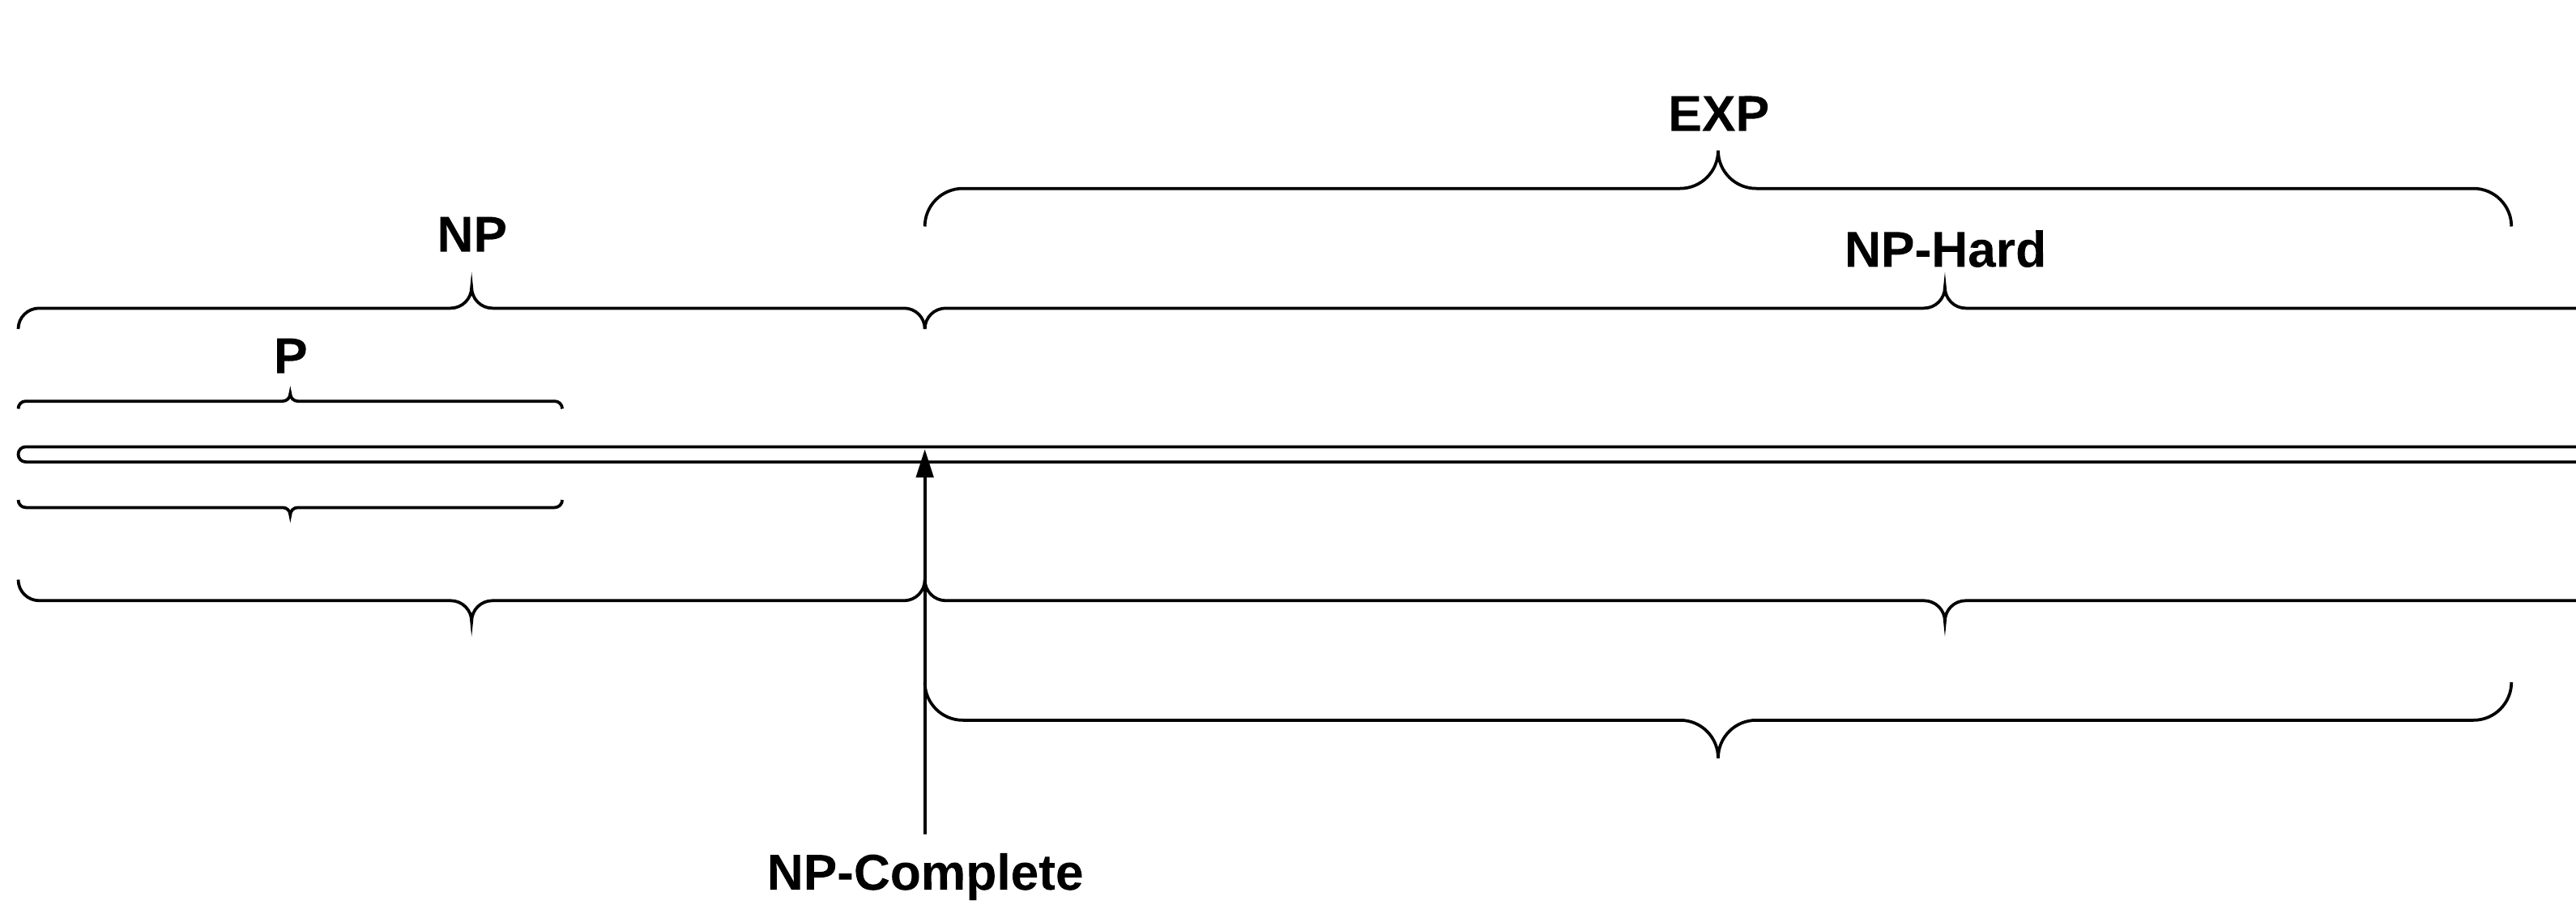
\includegraphics[scale=.75, angle = 90]{Time_Complexity_Line.png}
\end{center}

\begin{figure}
\centering
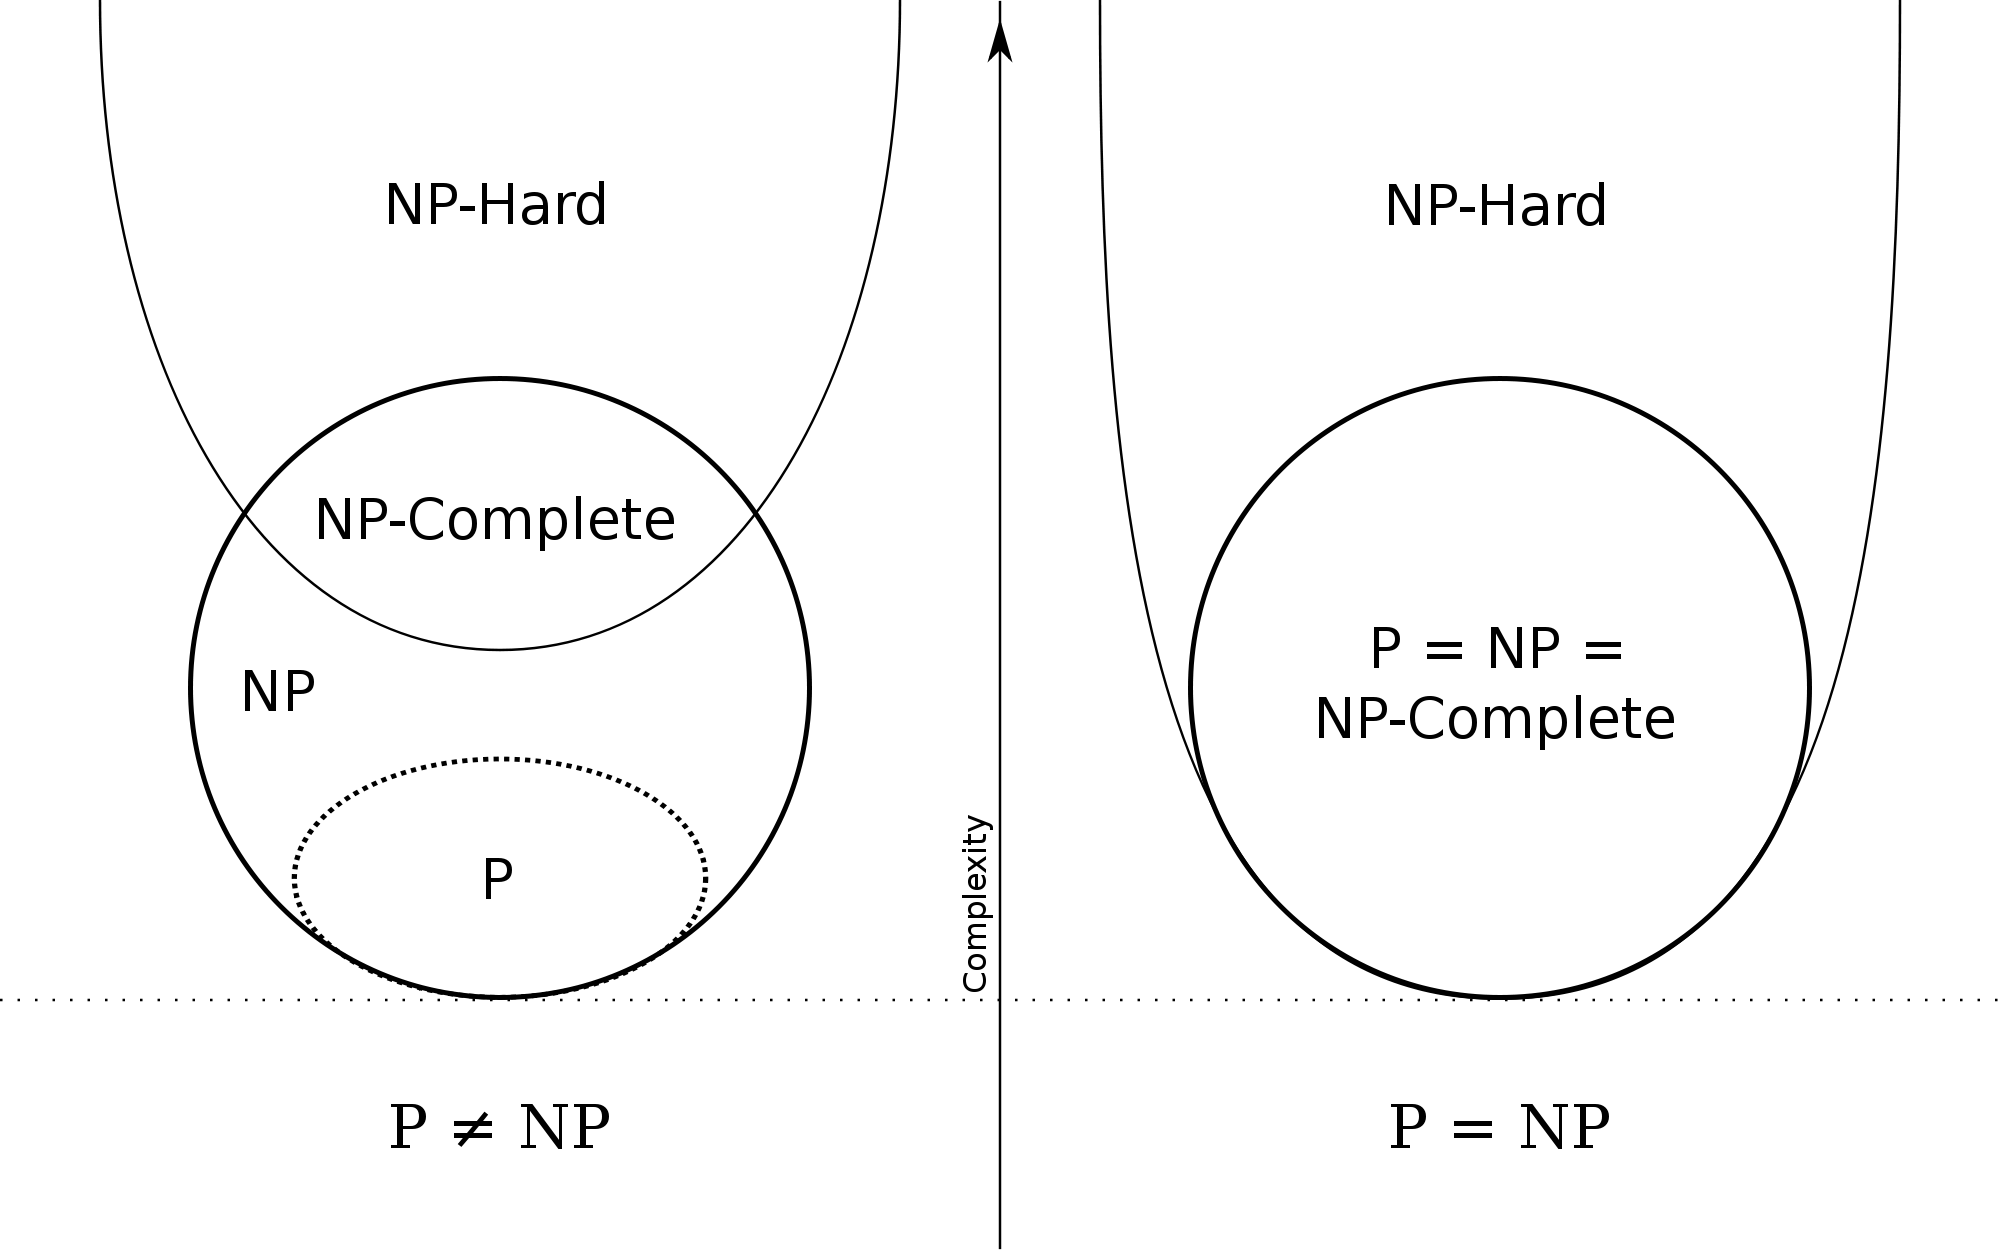
\includegraphics[scale=0.25]{P_vs_NP_Euler_Diagram}
\caption{Euler Diagram showing P vs NP vs NP-Hard}
\end{figure}
\newpage
\begin{figure}
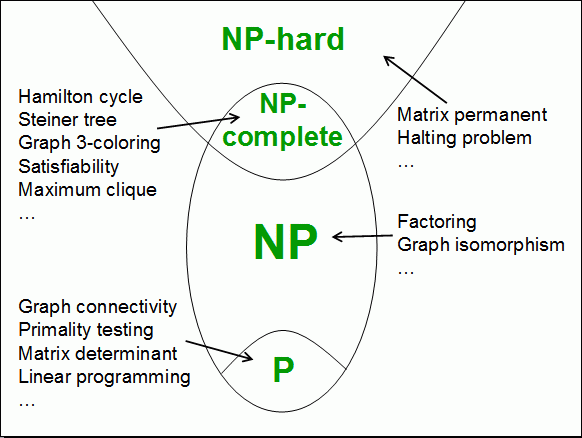
\includegraphics[scale=.8]{examples_time_complexity.png}
\caption{P, NP, NP-Hard Problems}
\end{figure}



\vspace*{1 cm}
\bibliographystyle{plain}
\bibliography{references}


\end{document}